\documentclass[tikz]{standalone}
\usetikzlibrary{positioning, arrows.meta, trees}
\begin{document}
    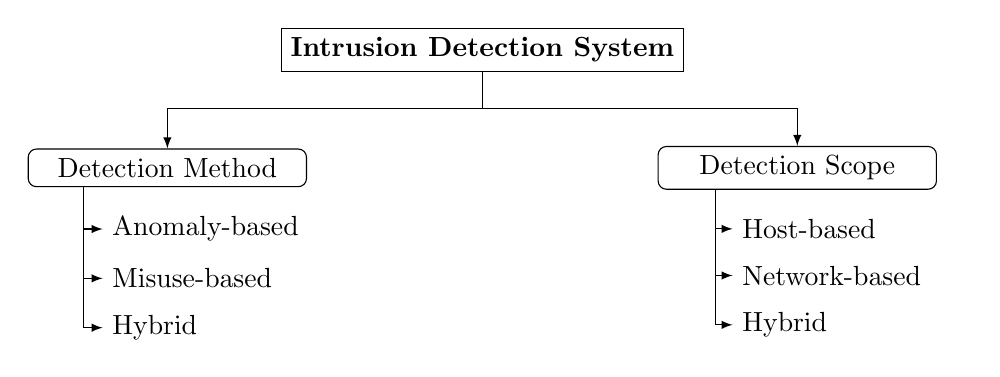
\begin{tikzpicture}
        [
            root/.style = {draw, black},
            level 1/.style = {draw, black, sibling distance = 8cm},
            edge from parent/.style={->,black,draw}, 
            edge from parent path={(\tikzparentnode.south) -- (\tikzchildnode.north)},
            >=latex, node distance=5.2cm, edge from parent fork down
        ]%
        \node[root] {\textbf{Intrusion Detection System}}
            child {node[level 1, rounded corners=3pt, align=center, text width=3.3cm] (method) {Detection Method}}
            child {node[level 1, rounded corners=3pt, align=center, text width=3.3cm] (scope) {Detection Scope}};
        \node [below = 0.25cm of method, xshift=20pt, text width=2.8cm] (anomaly) {Anomaly-based};
        \node [below = 0.1cm of anomaly, text width=2.8cm] (misuse) {Misuse-based};
        \node [below = 0.1cm of misuse, text width=2.8cm] (hybrid) {Hybrid};
        \draw[->] (method.193) |- (anomaly.west);
        \draw[->] (method.193) |- (misuse.west);
        \draw[->] (method.193) |- (hybrid.west);
        \node [below = 0.25cm of scope, xshift=20pt, text width=2.8cm] (host) {Host-based};
        \node [below = 0.1cm of host, text width=2.8cm] (network) {Network-based};
        \node [below = 0.1cm of network, text width=2.8cm] (hybrid2) {Hybrid};
        \draw[->] (scope.195) |- (host.west);
        \draw[->] (scope.195) |- (network.west);
        \draw[->] (scope.195) |- (hybrid2.west);
        \end{tikzpicture}
\end{document}